\documentclass{article}
\usepackage[margin=1in]{geometry} 
\usepackage{amsmath,amsthm,amssymb,amsfonts, fancyhdr, color, comment, graphicx, environ}
\usepackage{xcolor}
\usepackage{mdframed}
\usepackage[shortlabels]{enumitem}
\usepackage{indentfirst}
\usepackage{hyperref}
\hypersetup{
    colorlinks=true,
    linkcolor=blue,
    filecolor=magenta,      
    urlcolor=blue,
}
\usepackage{pgfplots}
\pgfplotsset{width=10cm,compat=1.9}
\pgfplotsset{compat=1.17}
\usepackage{tikz}
\usepackage{caption}

\setlength{\parindent}{0pt}


%for headers 
\pagestyle{fancy}
\fancyhf{} % for header/footer

\lhead{Creel}
\rhead{ENV 795 - Nature as Capital}
\chead{\textbf{Ecological Modeling}}

\title{Week Two - Ecological Modeling}
\author{Andie Creel for Nature as Capital}
\date{February 6th, 2023}


\begin{document}
\maketitle

\section{Changes through time}
Reminder: Capital stores wealth through time. That's why we need to model things through time.\\

Review from video:

\begin{itemize}
    \item Recursion equations: $x_{t+1} = f(x_t)$ OR $y = f(x)$ where $y$ is $x_{t+1}$ and $x$ is $x_t$
    \item Usually get the form: $x_{t+1} = x_t + g(x_t, z)$ where $g()$ is a growth equation and $z$ is some state.
    \item Difference equation (discrete time): $x_{t+1} - x_t = g(x_t, z)$
    \item Differential equation (continuous time):  $\frac{\partial x}{\partial t} = \dot x$
\end{itemize}

\subsection{Logistic Growth}

$$ \dot x = \frac{\partial x}{\partial t} = rx(1 - \frac{x}{K})$$

Where will $\dot x = 0$? There are 2 roots so there are 2 spots it will equal zero. It's already factored, so set each part equal to zero. 

$$ 1 - x/K = 0 \implies x_{ss} = K$$
$$ rx = 0 \implies x_{ss} = 0$$

When $x > 0$ but $ x < K$ we know the growth rate is positive. When $x > K$, the growth rate is negative. Therefore we known when $x_{ss} = K$ is a stable point, b/c if $x$ is perturbed, it will return to $K$. 

\subsection{Logistic Growth with Harvest}
$$ \dot x = rx(1 - x/K) - h$$
So long as $h$ is is less than the maximum sustainable yield, we're sustainable (where sustainable means we are not depleting the stock i.e. the stock is still growing, replenishing itself). Remember, sustainable means the stock isn't declining. But if the stock is at 0, "sustainable" may not be the goal. \\

If $h > rx(1-x/K)$, $\dot x <0$ and the population is decreasing. \\

This function is convex, area under the curve is a convex set. If you draw a line from the origin, it will only cross the function once. If the management policy is to harvest 10\%, you will only have one population level that you'll end up at, and \textbf{it will be stable.}

\begin{figure}[htp]
    \centering
    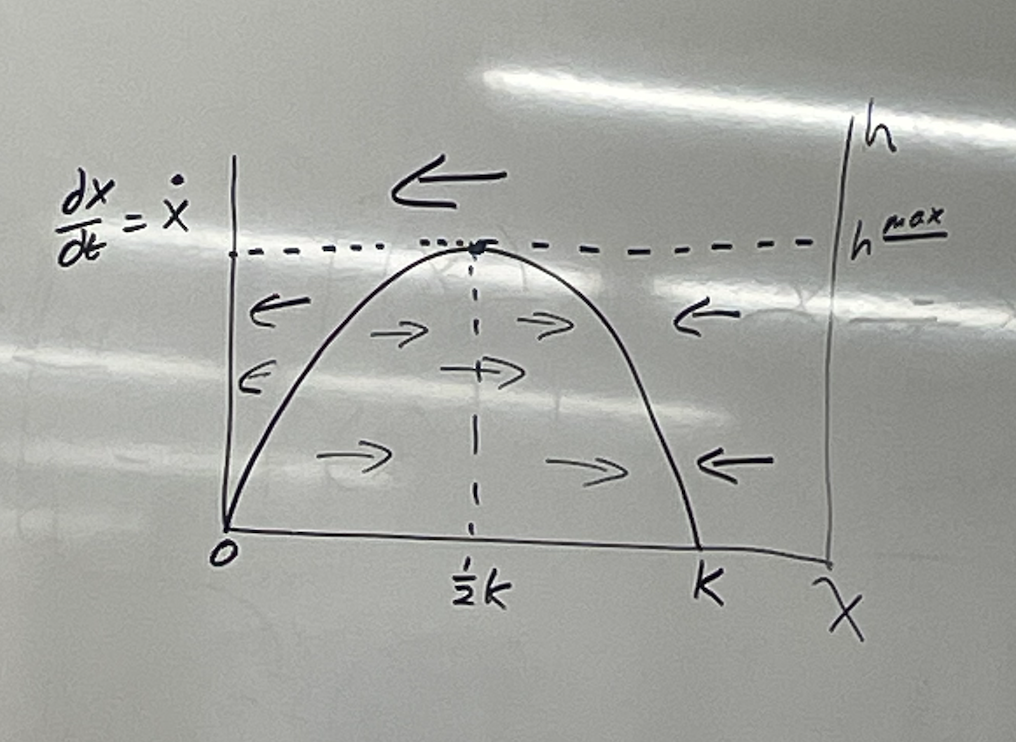
\includegraphics[width=9cm]{phase_plane.png}
    \caption{Phase plane for logistic growth}
\end{figure}


\subsection{Approximation}
\begin{itemize}
    \item zeroth order approximation: mean
    \item first order approx.: Linear regression
    \item Second order approx.: parabola 
\end{itemize}

\section{Allee affect: tipping points} 
$$\dot x = rx(\frac{x}{b} - 1)(1-\frac{x}{K})$$

$b$ will be the minimum viable population in ecology. Populations above $x > b$ will have a positive growth rate until $K$. But populations below $b$ will have negative growth. Note that $b$ is an unstable equilibrium. \\

This function is non-convex. It has tipping points/thresholds. Non-convexity are what introduce tipping points. To get a non-convexity, you need a higher order equation. But data to fit those models must be very very rich. If you draw a line from the origin, it will cross the line \textbf{twice}. Following a policy of "let's harvest 10\%" leads to two potential population level, \textbf{one of which will be unstable. }

\begin{figure}[htp]
    \centering
    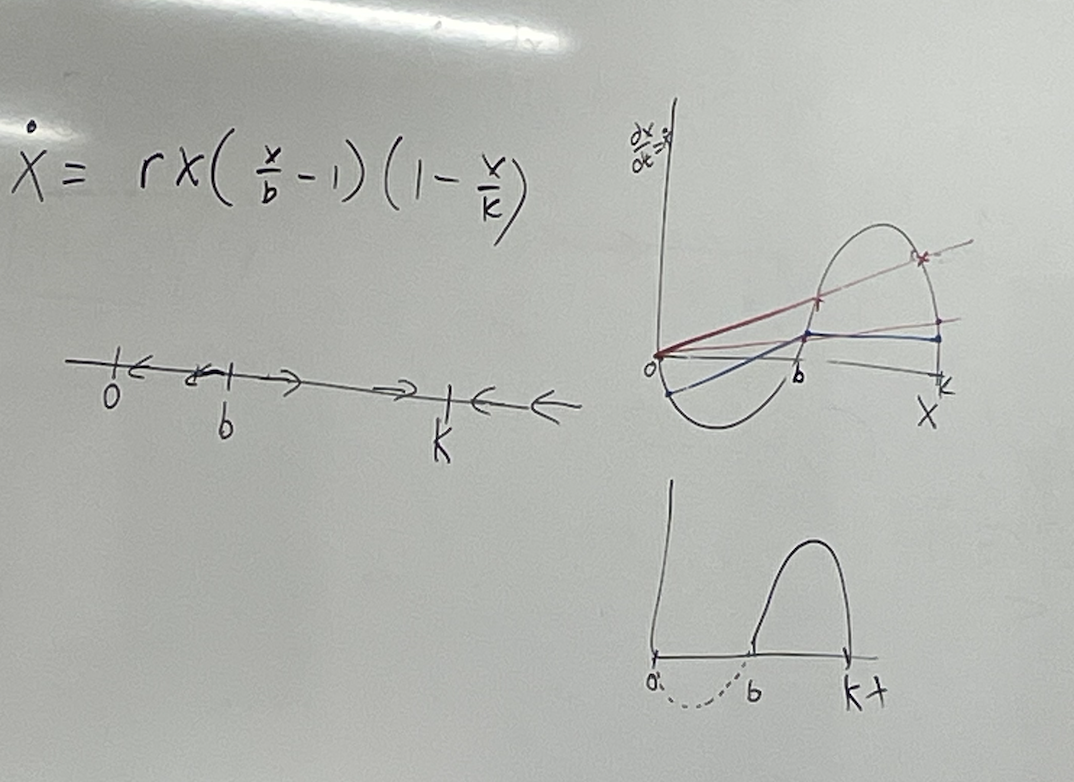
\includegraphics[width=7cm]{phase_plane_tip.png}
    \caption{Phase plane for allee effect}
\end{figure}

\section{Predator Prey System}

\subsection{Holling's Disk I Equation}
$x$ is prey, $y$ is predator. This is also an infectious disease model.

Prey's growth is slowed down by the presence of predators. They larger $y$ is, the smaller $\dot x$ is.
$$\dot x = rx - \alpha xy$$

Predators grow more, $\dot y$, when the population of prey, $x$, is higher.
$$\dot y = \beta xy - qy$$

$\alpha > \beta$ otherwise the predators are "making" more biomass than they eat (which is impossible). There needs to be some loss of energy. \\

\subsection{Null-cline/isoclines:}
We want to find a point where $\dot x $ and $\dot y$ are not changing (i.e., = 0). \\

Let's factor the prey's growth equation: 
$$\dot x = x(r-\alpha y).$$\\

We're not interested in prey population level equalling zero, $x_{ss} = 0$, so we known $\dot x$ is zero (population is stable) when $y = r/\alpha$. \\

Let's factor the predator growth equation: 
$$ \dot y = y(\beta x - q).$$
We're not interested in a case with no predators. So we know know $\dot y$ is zero (population isn't changing) when $x = q/ \beta$.

\begin{figure}[htp]
    \centering
    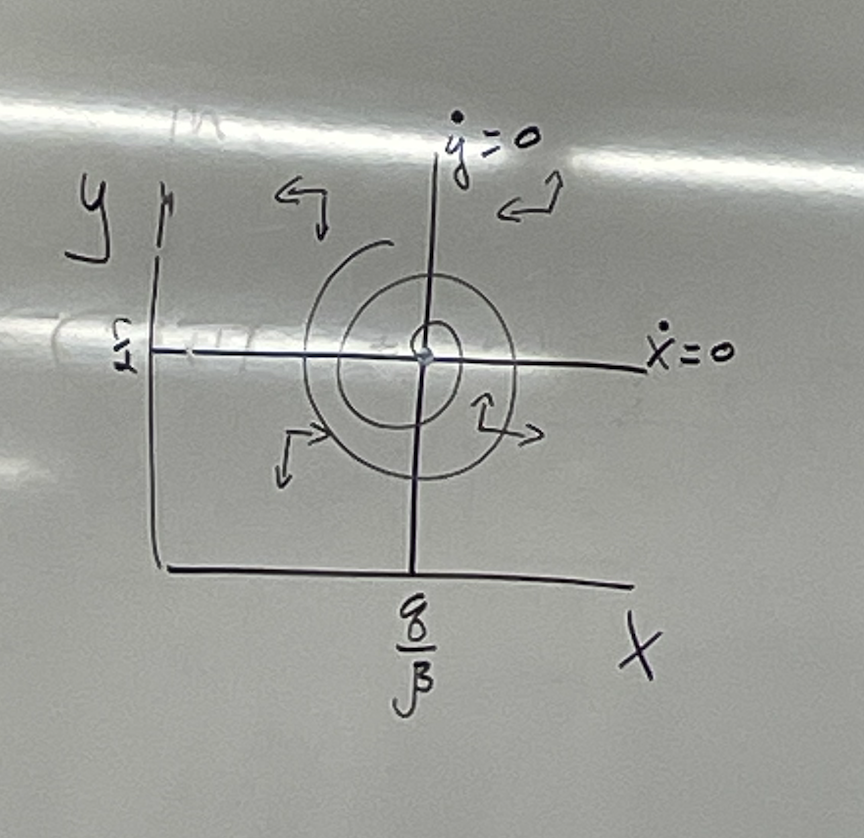
\includegraphics[width=7cm]{phase_plane_3.png}
    \caption{Phase plane for holling disk I}
\end{figure}

\subsection{Holling's Disk II Equation}
Predators get full. \\

\textbf{Recursion equation for prey:}
$$X_{t+1} = r X_t (1 - \frac{X_t}{K}) - \frac{C X_t}{D + X_t}* Y_t + X_t$$
Where $r$ is intrinsic growth rate, $K$ is the carrying capacity for prey, $C$ is the predators max consumption rate, and $D$ is the half saturation rate. \\

\textbf{Difference Eqn for prey:}
$$\dot X_t = X_{t+1} - X_t = r X_t (1 - \frac{X_t}{K}) - \frac{C X_t}{D + X_t}* Y_t $$

\textbf{Recursion equation for predator:}
$$Y_{t+1} = \frac{\beta(CX_t)}{D + X_t}*Y_t - mY_t - \alpha Y_t + Y_t$$
where $\beta$ is the conversion efficiency rate, $m$ is the mortality rate, and $\alpha$ is the harvest rate of \textit{predators}. \\

\textbf{Difference Eqn of predator:}
$$\dot Y_t = Y_{t+1} = \frac{\beta(CX_t)}{D + X_t}*Y_t - mY_t - \alpha Y_t$$





\subsection{Holling's Disk III Equation}
Change $\alpha x$ to $\frac{K x^2}{D^2 + x^2}$ where $D = 1 / \alpha h$ and $K = 1/h$. 
\begin{figure}[htp]
    \centering
    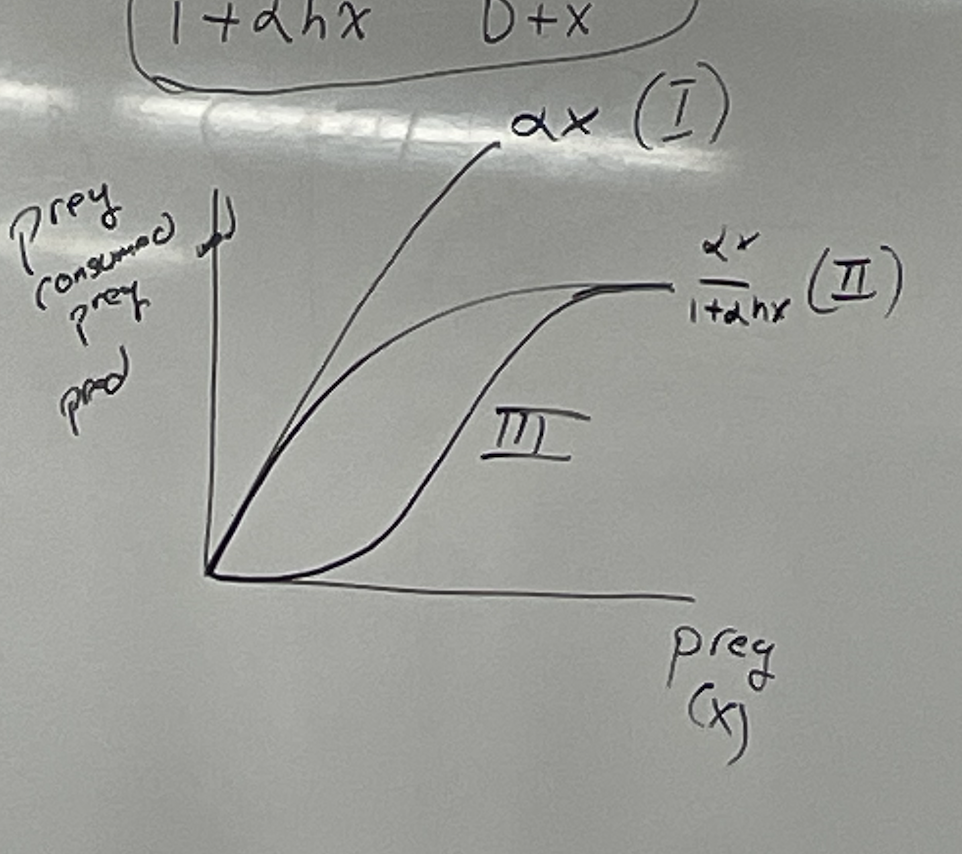
\includegraphics[width=7cm]{holling-disk.png}
    \caption{Three types of Holling Disk}
\end{figure}

\section{Resource Sharing}
Two animals are consuming the same food source. Both animal $x$ and $y$ eat it. So they affect one anther's growth rate through resource competition. 

$$ \dot x = rx(1 - \frac{x + \alpha y}{K})$$

$$ \dot y = b y ( 1 - \frac{\beta x + y}{J})$$

\section{Back to tipping points}
Holling type III and resource sharing: crayfish and bass. Some of Eli's old work.

$$ \dot x = x(1 - x - \alpha y) - \frac{\delta - y x^2}{K^2 - x^2}$$

$$\dot y = ry(1 - \beta x - y) + \frac{\epsilon \delta y x^2}{K^2 - x^2}$$

\begin{figure}[htp]
    \centering
    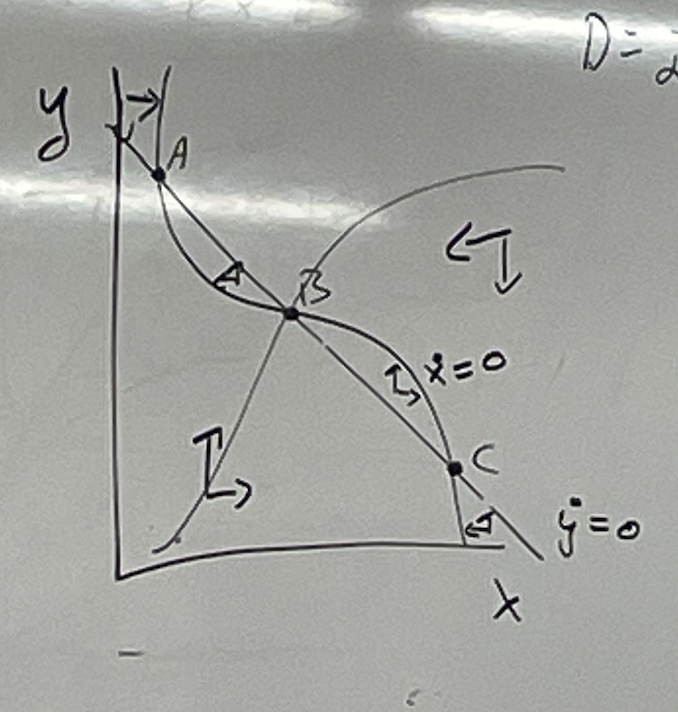
\includegraphics[width=7cm]{bass-crayfish.png}
    \caption{Eli's old work}
\end{figure}


\end{document}